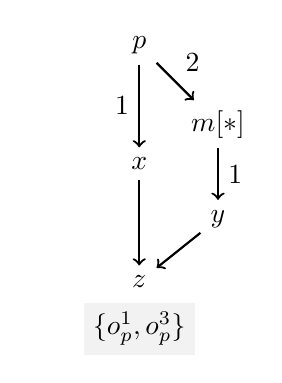
\begin{tikzpicture}[scale=1,thick]
    \node (p) at (0, 0) {$\textpurple{p}$};
    \node (x) at (0, -1.5) {$x$};
    \node (m) at (1, -1) {$m[*]$};
    \node (y) at (1, -2.2) {$y$};
    \node (z) at (0, -3) {$z$};

    \draw [->] (p) --node[left]{$1$} (x);
    \draw [->] (x) -- (z);
    \draw [->] (p) --node[above right]{$2$} (m);
    \draw [->] (m) --node[right]{$1$} (y);
    \draw [->] (y) -- (z);

    \node at (-1.3, 0) {};

    \node[fill=gray!10] (t) at (0, -3.6) {$\{o_p^1, o_p^3\}$};
\end{tikzpicture}
